%% Creator: Inkscape 1.2.2 (b0a84865, 2022-12-01), www.inkscape.org
%% PDF/EPS/PS + LaTeX output extension by Johan Engelen, 2010
%% Accompanies image file 'res/paradoxeSpanungsmessung2.pdf' (pdf, eps, ps)
%%
%% To include the image in your LaTeX document, write
%%   \input{<filename>.pdf_tex}
%%  instead of
%%   \includegraphics{<filename>.pdf}
%% To scale the image, write
%%   \def\svgwidth{<desired width>}
%%   \input{<filename>.pdf_tex}
%%  instead of
%%   \includegraphics[width=<desired width>]{<filename>.pdf}
%%
%% Images with a different path to the parent latex file can
%% be accessed with the `import' package (which may need to be
%% installed) using
%%   \usepackage{import}
%% in the preamble, and then including the image with
%%   \import{<path to file>}{<filename>.pdf_tex}
%% Alternatively, one can specify
%%   \graphicspath{{<path to file>/}}
%% 
%% For more information, please see info/svg-inkscape on CTAN:
%%   http://tug.ctan.org/tex-archive/info/svg-inkscape
%%
\begingroup%
\def\svgwidth{\textwidth}
\makeatletter%
\providecommand\color[2][]{%
	\errmessage{(Inkscape) Color is used for the text in Inkscape, but the package 'color.sty' is not loaded}%
	\renewcommand\color[2][]{}%
}%
\providecommand\transparent[1]{%
	\errmessage{(Inkscape) Transparency is used (non-zero) for the text in Inkscape, but the package 'transparent.sty' is not loaded}%
	\renewcommand\transparent[1]{}%
}%
\providecommand\rotatebox[2]{#2}%
\newcommand*\fsize{\dimexpr\f@size pt\relax}%
\newcommand*\lineheight[1]{\fontsize{\fsize}{#1\fsize}\selectfont}%
\ifx\svgwidth\undefined%
	\setlength{\unitlength}{829.5867199bp}%
	\ifx\svgscale\undefined%
		\relax%
	\else%
		\setlength{\unitlength}{\unitlength * \real{\svgscale}}%
	\fi%
\else%
	\setlength{\unitlength}{\svgwidth}%
\fi%
\global\let\svgwidth\undefined%
\global\let\svgscale\undefined%
\makeatother%
\begin{picture}(1,0.42492613)%
	\lineheight{1}%
	\setlength\tabcolsep{0pt}%
	\put(0,0){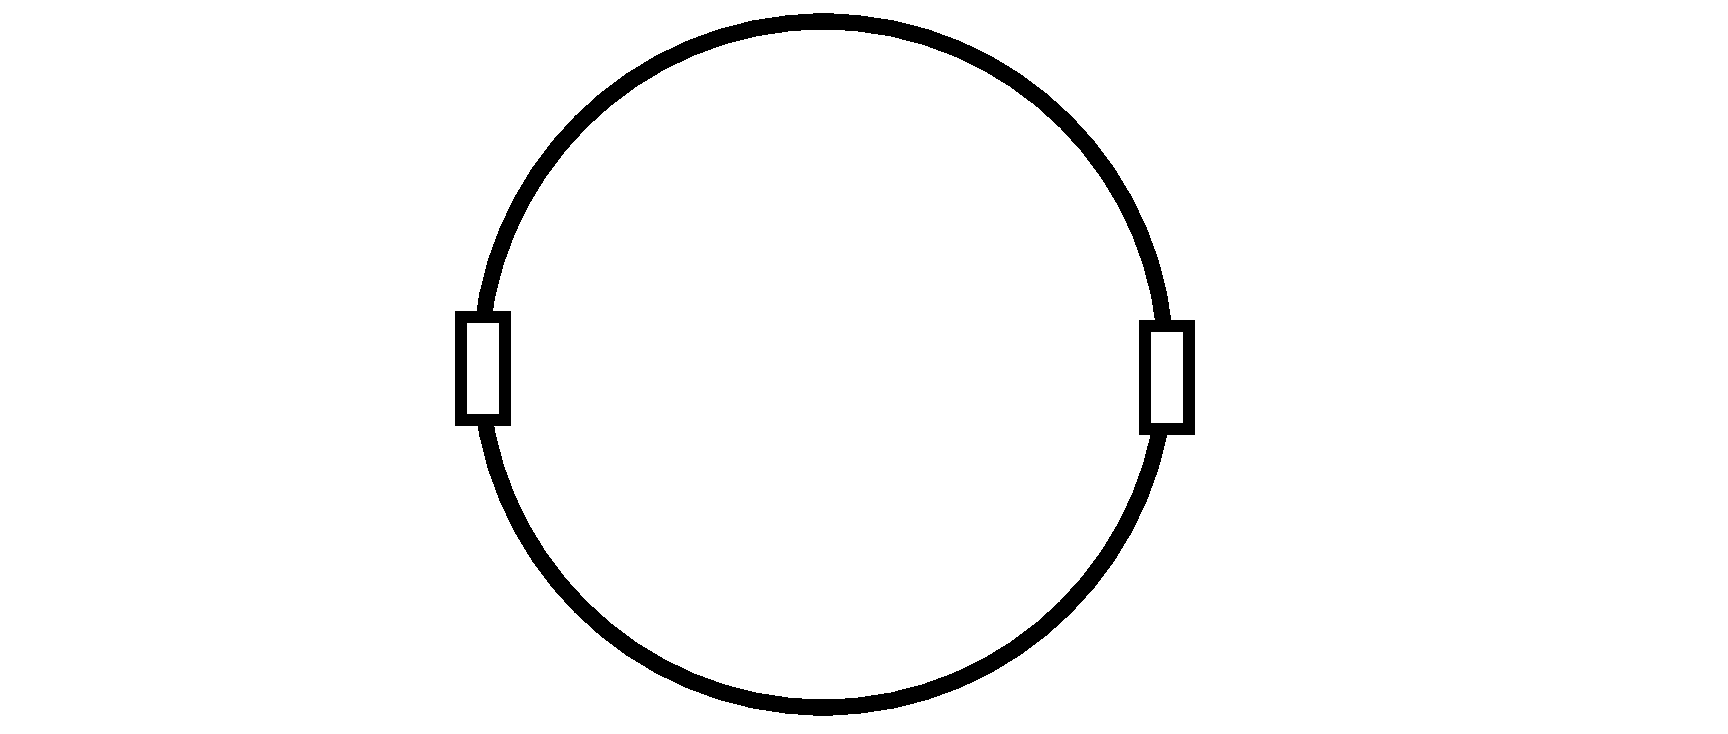
\includegraphics[width=\unitlength,page=1]{res/paradoxeSpanungsmessung2.pdf}}%
	\put(0.7045381,0.1983655){\color[rgb]{0,0,0}\makebox(0,0)[lt]{\lineheight{1.25}\smash{\begin{tabular}[t]{l}$R_2$\end{tabular}}}}%
	\put(0.21171265,0.20167302){\color[rgb]{0,0,0}\makebox(0,0)[lt]{\lineheight{1.25}\smash{\begin{tabular}[t]{l}$R_1$\end{tabular}}}}%
	\put(0.39689155,0.27113165){\color[rgb]{0,0,0}\makebox(0,0)[lt]{\lineheight{1.25}\smash{\begin{tabular}[t]{l}$-\frac{\partial \vec{B}}{\partial t}$\end{tabular}}}}%
	\put(0,0){\includegraphics[width=\unitlength,page=2]{res/paradoxeSpanungsmessung2.pdf}}%
	\put(0.06575846,0.1971287){\color[rgb]{0,0,0}\makebox(0,0)[lt]{\lineheight{1.25}\smash{\begin{tabular}[t]{l}$U_1$\end{tabular}}}}%
	\put(0.85150847,0.20341783){\color[rgb]{0,0,0}\makebox(0,0)[lt]{\lineheight{1.25}\smash{\begin{tabular}[t]{l}$U_2$\end{tabular}}}}%
	\put(0.31981416,0.15056218){\color[rgb]{0,0,0}\makebox(0,0)[lt]{\lineheight{1.25}\smash{\begin{tabular}[t]{l}$\mathcal{E}=\oint\limits_{C(A)} \vec{E}\cdot \dd \vec{s} = -\iint\limits_A \dot{\vec{B}}\cdot \dd \vec{A}$\end{tabular}}}}%
	\put(0.32846175,0.32194138){\color[rgb]{0,0,0}\makebox(0,0)[lt]{\lineheight{1.25}\smash{\begin{tabular}[t]{l}$\mathcal{E}/4$\end{tabular}}}}%
	\put(0.35204605,0.07666474){\color[rgb]{0,0,0}\makebox(0,0)[lt]{\lineheight{1.25}\smash{\begin{tabular}[t]{l}$\mathcal{E}/4$\end{tabular}}}}%
	\put(0.57137998,0.08374004){\color[rgb]{0,0,0}\makebox(0,0)[lt]{\lineheight{1.25}\smash{\begin{tabular}[t]{l}$\mathcal{E}/4$\end{tabular}}}}%
	\put(0.56666313,0.33137513){\color[rgb]{0,0,0}\makebox(0,0)[lt]{\lineheight{1.25}\smash{\begin{tabular}[t]{l}$\mathcal{E}/4$\end{tabular}}}}%
	\put(0.19481742,0.31329384){\color[rgb]{0,0,0}\makebox(0,0)[lt]{\lineheight{1.25}\smash{\begin{tabular}[t]{l}$\mathcal{E}/4$\end{tabular}}}}%
	\put(0.19560356,0.10889662){\color[rgb]{0,0,0}\makebox(0,0)[lt]{\lineheight{1.25}\smash{\begin{tabular}[t]{l}$\mathcal{E}/4$\end{tabular}}}}%
	\put(0.69873519,0.08924303){\color[rgb]{0,0,0}\makebox(0,0)[lt]{\lineheight{1.25}\smash{\begin{tabular}[t]{l}$\mathcal{E}/4$\end{tabular}}}}%
	\put(0.69637676,0.33058898){\color[rgb]{0,0,0}\makebox(0,0)[lt]{\lineheight{1.25}\smash{\begin{tabular}[t]{l}$\mathcal{E}/4$\end{tabular}}}}%
\end{picture}%
\endgroup%
